\begin{exercise}
\begin{figure}[H]
\centering
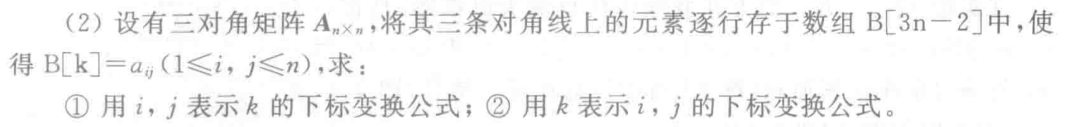
\includegraphics[width=\textwidth]{hw4-2025042916.png}
% \caption{}
\label{}
\end{figure}
\end{exercise}
1️⃣
\[
(i,j)\longmapsto k=j+2i-3
\]
2️⃣
\[
k\longmapsto(i,j)=\left( \left[ \frac{k+1}{3} \right]+1,k+1-2\left[ \frac{k+1}{3} \right] \right)
\]
\begin{exercise}
\begin{figure}[H]
\centering
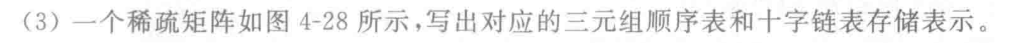
\includegraphics[width=\textwidth]{1-hw4-2025042916.png}
% \caption{}
\label{}
\end{figure}
\begin{figure}[H]
\centering
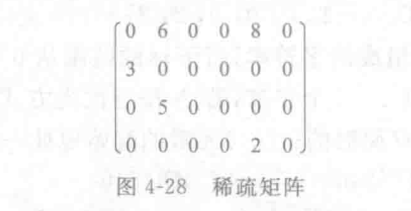
\includegraphics[width=\textwidth]{2-hw4-2025042916.png}
% \caption{}
\label{}
\end{figure}
\end{exercise}
\begin{figure}[H]
\centering
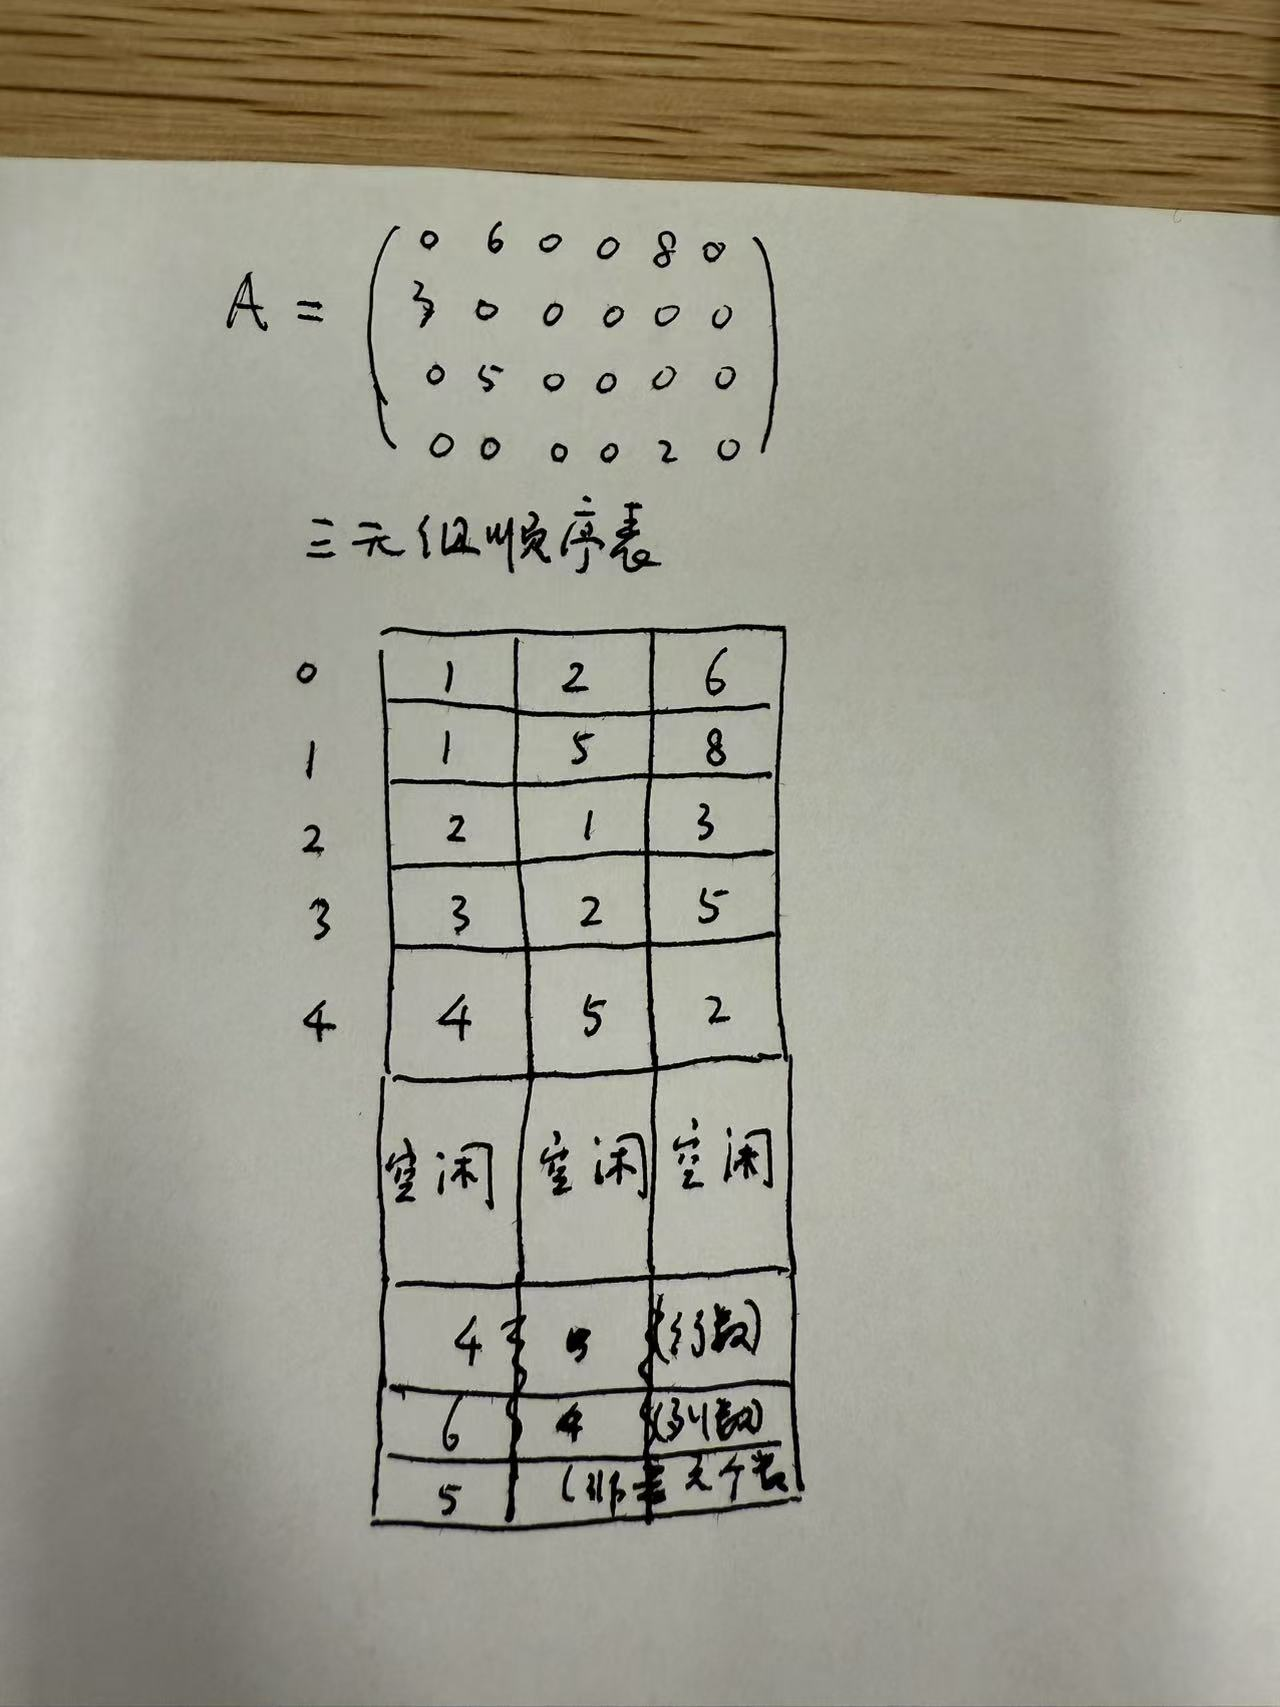
\includegraphics[width=\textwidth]{36f98016793f2f6411957091dd1eb9f9.jpg}
% \caption{}
\label{}
\end{figure}
\begin{figure}[H]
\centering
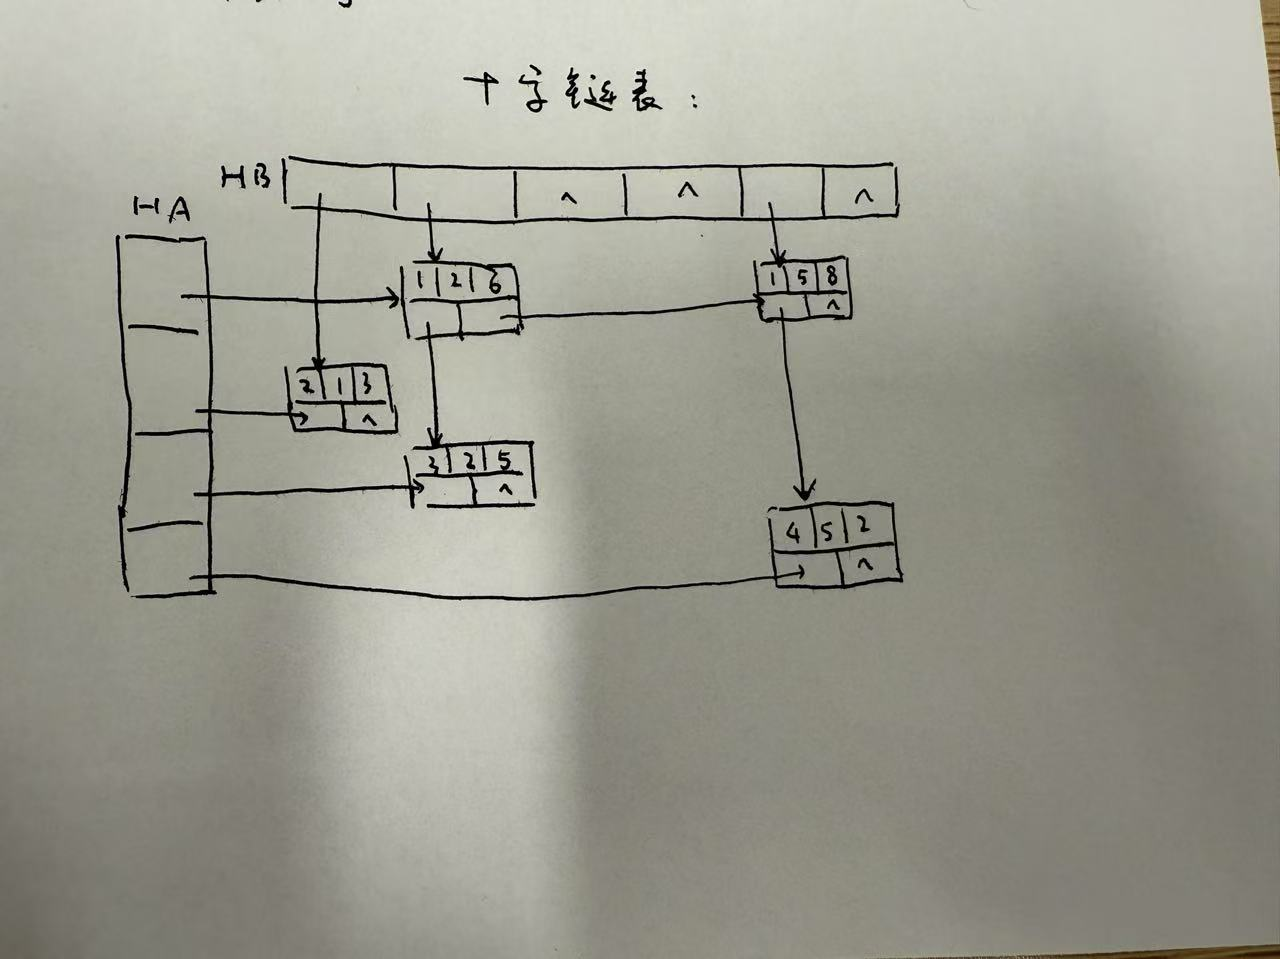
\includegraphics[width=\textwidth]{1a1ff436b1cc74c417a289bd3d98be7c.jpg}
% \caption{}
\label{}
\end{figure}

\begin{exercise}
\begin{figure}[H]
\centering
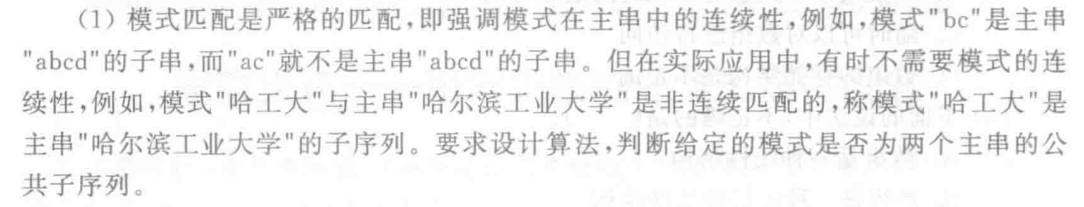
\includegraphics[width=\textwidth]{3-hw4-2025042916.png}
% \caption{}
\label{}
\end{figure}
\end{exercise}
\begin{lstlisting}[language=C++]
#include <iostream>
#include <string>

using namespace std;

bool isSubsequence(const string& pattern, const string& text) {
  int len_pattern = pattern.length();
  int len_text = text.length();
  int p_pattern = 0;
  int p_text = 0;

  while (p_pattern < len_pattern && p_text < len_text) {
    if (pattern[p_pattern] == text[p_text]) {
      p_pattern++;
    }
    p_text++;
  }

  return p_pattern == len_pattern;
}

int main() {
  string pattern = "哈工大";
  string text1 = "哈尔滨工业大学";
  string text2 = "我们热爱哈尔滨工业大学";

  if (isSubsequence(pattern, text1) && isSubsequence(pattern, text2)) {
    cout << pattern + " 是 " + text1 + " 和 " + text2 + " 的公共子序列" << endl;
  } else {
    cout << pattern + " 不是 " + text1 + " 和 " + text2 + " 的公共子序列" << endl;
  }

  return 0;
}
\end{lstlisting}
\begin{exercise}
\begin{figure}[H]
\centering
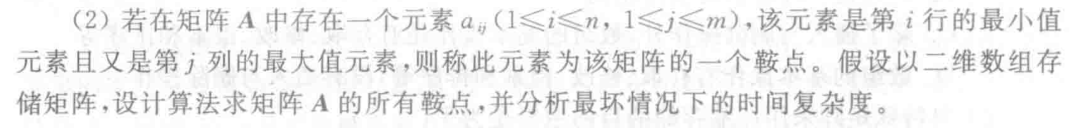
\includegraphics[width=\textwidth]{4-hw4-2025042916.png}
% \caption{}
\label{}
\end{figure}
\end{exercise}
先找到每一行的最小值元素,再将这个元素和该列所有元素比较,若为最大值元素,则输出位置.

\begin{lstlisting}
for i = 0 to n-1:
    min_val = A[i][0]
    min_col = 0
    for j = 1 to m-1:
        if A[i][j] < min_val:
            min_val = A[i][j]
            min_col = j

    is_saddle = true
    for k = 0 to n-1:
        if A[k][min_col] > min_val:
            is_saddle = false
            break

    if is_saddle:
        print("Saddle point at (", i, ",", min_col, ") with value", min_val)

\end{lstlisting}
时间复杂度为 $O(mn+n^2)$.

\begin{exercise}
\begin{figure}[H]
\centering
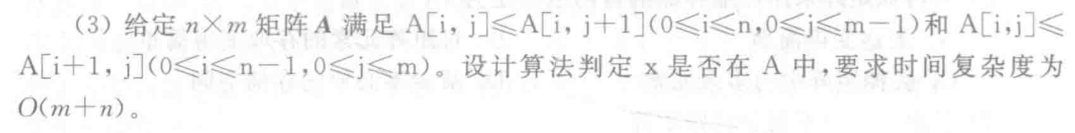
\includegraphics[width=\textwidth]{5-hw4-2025042916.png}
% \caption{}
\label{}
\end{figure}
\end{exercise}
\textbf{核心思想(从右上角开始搜索)}

从\textbf{右上角}开始(\lstinline{i = 0, j = m-1}):

\begin{itemize}
	\item 如果 $A[i][j] == x$,则找到,返回 true。
	\item 如果 $A[i][j] > x$,则说明 $x$ 一定不在这一列,左移(\lstinline{j -= 1})。
	\item 如果 $A[i][j] < x$,则说明 $x$ 一定不在这一行,向下移(\lstinline{i += 1})。
\end{itemize}

\begin{lstlisting}
def search_matrix(A, x):
    n = len(A)
    m = len(A[0])
    i = 0
    j = m - 1
    while i < n and j >= 0:
        if A[i][j] == x:
            return True
        elif A[i][j] > x:
            j -= 1
        else:
            i += 1
    return False

\end{lstlisting}
\begin{itemize}
	\item 最多移动 $n$ 次向下、$m$ 次向左,因此最多执行 $n + m$ 次比较。
	\item 时间复杂度是 $\boxed{O(n + m)}$,满足题设要求。
\end{itemize}
